\subsubsection{Optimisation for Deep Learning}

\begin{remark} \hlt{Optimisation}\\
A cost function $J(\bm{\theta})$ is reduced to improve some performance measure $P$.\\
Optimisation algorithms include some specialisation on specific structure of machine learning objective functions.\\
Cost function is average over training set,
\begin{equation}
J(\bm{\theta}) = \mathbb{E}_{(\bm{x}, y) \sim \hat{p}_{\text{data}}} L(f(\bm{x}; \bm{\theta}), y) \nonumber
\end{equation}
where $L$ is per-example loss function, $f(\bm{x}; \bm{\theta})$ is predicted output given input $\bm{x}$, $\hat{p}_{\text{data}}$ is empirical distribution. For supervised learning, $y$ is target output.\\
The goal is to usually to minimise objective function where expectation is taken on data generating distribution $p_{\text{data}}$ rather than over the finite training set:
\begin{equation}
J^*(\bm{\theta}) = \mathbb{E}_{(\bm{x}, y) \sim p_{\text{data}}} L(f(\bm{x}; \bm{\theta}), y) \nonumber
\end{equation}
Note that machine learning algorithm usually minimises a surrogate loss function, and halts when convergence criterion based on early  stopping is satisfied.
\end{remark}

\begin{definition} \hlt{Empirical Risk Minimisation}\\
To minimise expected loss on training set, where $\hat{p}(\bm{x}, y)$ is the empirical distribution. The empirical risk is
\begin{equation}
\mathbb{E}_{\bm{x}, y \sim \hat{p}_{\text{data}}(\bm{x}, y)}[L(f(\bm{x}, \bm{\theta}), y)] = \frac{1}{m} \sum\limits_{i=1}^m L(f(\bm{x}^{(i)}; \bm{\theta}), y^{(i)}) \nonumber
\end{equation}
where $m$ is number of training samples. Note that empirical risk minimisation is prone to overfitting, as models with high capacity may memorise the training set.
\end{definition}

\begin{remark} \hlt{Batch and Minibatch Algorithms}\\
Objective algorithms for machine learning computes each update to the parameters based on expected value of cost function using only a subset of terms of full cost function.\\
For maximum likelihood estimation problems, note that
\begin{align}
\bm{\theta}_{\text{ML}} &= \arg \max_{\bm{\theta}} \sum\limits_{i=1}^m \log p_{\text{model}}(\bm{x}^{(i)}, y^{(i)}; \bm{\theta}) \nonumber \\
J(\bm{\theta}) &= \mathbb{E}_{\bm{x}, y \sim \hat{p}_{\text{data}}} \log p_{\text{model}} (\bm{x}, y; \bm{\theta}) \nonumber
\end{align}
The gradient is then
\begin{equation}
\nabla_{\bm{\theta}} J(\bm{\theta}) = \mathbb{E}_{\bm{x}, y \sim \hat{p}_{\text{data}}} \nabla_{\bm{\theta}} \log \log p_{\text{model}} (\bm{x}, y; \bm{\theta}) \nonumber
\end{equation}
If the optimisation algorithm uses the entire training set, then it is a batch gradient method.\\
If a single sample is used at a time, then this is a stochastic/online gradient method.\\
For algorithms that uses more than one but less than all samples, then this is a minibatch gradient method.
\end{remark}

\begin{remark} \hlt{Challenges: Ill-Conditioning of Hessian Matrix $H$}\\
May cause stochastic gradient descent to be stuck where very small step increases the cost function.\\
Note that a gradient descent step of $- \bm{\epsilon} \bm{g}$ will add
\begin{equation}
\frac{1}{2} \epsilon^2 \bm{g}^T \bm{H} \bm{g} - \epsilon \bm{g}^T \bm{g} \nonumber
\end{equation}
to the cost. This will be a problem when $\frac{1}{2} \epsilon^2 \bm{g}^T \bm{H} \bm{g} > \epsilon \bm{g}^T \bm{g}$.\\
Monitor squared gradient norm $\bm{g}^T \bm{g}$ and $\bm{g}^T \bm{H} \bm{g}$ term. When ill-conditioning happens, gradient norm does not shrink significantly but $\bm{g}^T \bm{H} \bm{g}$ term grows more than order of magnitude, and learning rate shrinks.
\end{remark}

\begin{remark} \hlt{Challenges: Local Minimums}\\
Neural networks and models with multiple parametrised latent variables have multiple local minima due to \hlt{model identifiability} problem. Model is identifiable if a sufficiently large training set can rule out all but one setting of model parameters. Models with latent variables are not identifiable as equivalent models are obtained by exchanging latent variables with each other (\hlt{weight space symmetry}). If there are $m$ layers with $n$ units each, then there are $n!^m$ ways to arrange the hidden units, making the model unidentifiable.\\
There may be an extremely large or uncountably infinite amount of local minima in a cost function. If the local minima have a high cost compared to global minimum, then this is problematic.
\end{remark}

\begin{remark} \hlt{Challenges: Plateaus, Saddle Points, Flat Regions}\\
For a function $f: \R^n \rightarrow \R$, expected ratio of saddle points to local minima grows exponentially with $n$. Hessian matrix at a saddle point has a mixture of positive and negative eigenvalues.\\
Degenerate regions with flat gradient may correspond to high value of objective function.
\end{remark}

\begin{remark} \hlt{Challenges: Cliffs and Exploding Gradients}\\
On extremely steep cliff structure, gradient update step may move parameters extremely far, losing most of the optimisation work done previously. The consequences may be mitigated using gradient clipping heuristics, which reduces the step size to be small enough.
\end{remark}

\begin{remark} \hlt{Challenges: Long-Term Dependencies}\\
Occurs when computational graph becomes very deep. Let a computational graph contain a path that repeatedly multiply a matrix $\bm{W}$. After $t$ steps, this is $\bm{W}^t$. Let the eigen-decomposition of $\bm{W}$ be $\bm{W} = \bm{V} \text{diag}(\bm{\lambda}) \bm{V}^{-1}$. Then we can see that $\bm{W}^t = (\bm{V} \text{diag}(\bm{\lambda}) \bm{V}^{-1})^t = \bm{V} \text{diag}(\lambda)^t \bm{V}^{-1}$.\\
There will be a vanishing and exploding gradient problem if gradients on the graph are scaled according to $\text{diag}(\bm{\lambda})^t$.  Note that recurrent networks uses same $\bm{W}$ at each time step, hence may face the problem.
\end{remark}

\begin{remark} \hlt{Challenges: Inexact Gradients}\\
Objective function for minimisation is intractable due to noisy/biased estimate of these quantities; in this case its gradient is intractable as well. Choose surrogate loss function that is easier to approximate than true loss.
\end{remark}

\begin{remark} \hlt{Challenges: Poor Correspondence between Local and Global Structure}\\
As gradient descent algorithms make small local moves, optimisation on local downhill moves may fail if local surface does not point toward the global solution. In higher dimensional space, learning algorithms may incur high costs or long training time to circumnavigate the manifold. Hence to find good initial points for problems.
\end{remark}

\begin{remark} \hlt{Stochastic Gradient Descent (SGD)}\\
Crucial parameter is the learning rate, which may be changed over time; at iteration $k$ this is $\epsilon_k$.\\
The SGD gradient estimation introduces a source of noise that does not vanish even at minimum. A sufficient condition to guarantee converge of SGD is
\begin{equation}
\sum\limits_{k=1}^{\infty} \epsilon_k = \infty, \ \ \ \sum\limits_{k=1}^{\infty} \epsilon_k^2 < \infty \nonumber
\end{equation}
In practice, it is common to decay learning rate linearly until iteration $\tau$:
\begin{equation}
\epsilon_k = (1- \alpha)\epsilon_0 + \alpha \epsilon_{\tau}, \ \ \ \alpha = \frac{k}{\tau} \nonumber
\end{equation}
After iteration $\tau$, leave $\epsilon$ constant.\\
Compute time per update does not growth with number of training examples.
\end{remark}

\begin{breakablealgorithm}
\caption{Stochastic Gradient Descent (SGD) Update at Training Iteration $k$}
\begin{algorithmic}
\Require \\
Learning rate $\epsilon_k$, Initial parameter $\bm{\theta}$\\

\While {stopping criterion not met}
\State Sample a minibatch of $m$ samples from the training set $\{\bm{x}^{(1)}, \ldots, \bm{x}^{(m)} \}$ with targets $\bm{y}^{(i)}$
\State Compute gradient estimate $\hat{\bm{g}} \leftarrow + \frac{1}{m} \nabla_{\bm{\theta}} \sum_{i} L(f(\bm{x}^{(i)}; \bm{\theta}), \bm{y}^{(i)})$
\State Apply update: $\bm{\theta} \leftarrow \bm{\theta} - \epsilon \hat{\bm{g}}$
\EndWhile
\end{algorithmic}
\end{breakablealgorithm}

\begin{remark} \hlt{Momentum Algorithm}\\
Algorithm introduces variable $\bm{v}$ that is set to an exponentially decaying average of negative gradient.\\
Hyperparameter $\alpha \in [0, 1)$ determines how quickly the contributions of previous gradients exponentially decay.\\
The update rule is given by
\begin{align}
\bm{v} &\leftarrow \alpha \bm{v} - \epsilon \nabla_{\bm{\theta}} \left(\frac{1}{m} \sum\limits_{i=1}^m L(\bm{f}(\bm{x}^{(i)}; \bm{\theta}), \bm{y}^{(i)}) \right) \nonumber \\
\bm{\theta} &\leftarrow \bm{\theta} + \bm{v} \nonumber
\end{align}
The larger $\alpha$ is relative to $\epsilon$, the more previous gradients affect current direction.\\
If gradient is $\bm{g}$, it will accelerate in direction of $-\bm{g}$ until reaching terminal velocity where size of each step is
\begin{align}
\frac{\epsilon \norm{\bm{g}}}{1 - \alpha} \nonumber
\end{align}
\end{remark}

\begin{breakablealgorithm}
\caption{Stochastic Gradient Descent (SGD) with Momentum}
\begin{algorithmic}
\Require \\
Learning rate $\epsilon_k$, Momentum parameter $\alpha$\\

\While {stopping criterion not met}
\State Sample a minibatch of $m$ samples from the training set $\{\bm{x}^{(1)}, \ldots, \bm{x}^{(m)} \}$ with targets $\bm{y}^{(i)}$
\State Compute gradient estimate $\bm{g} \leftarrow + \frac{1}{m} \nabla_{\bm{\theta}} \sum_{i} L(f(\bm{x}^{(i)}; \bm{\theta}), \bm{y}^{(i)})$
\State Compute velocity update: $\bm{v} \leftarrow \alpha \bm{v} - \epsilon \bm{g}$
\State Apply update: $\bm{\theta} \leftarrow \bm{\theta} + \bm{v}$
\EndWhile
\end{algorithmic}
\end{breakablealgorithm}

\begin{figure}[H]
\centering
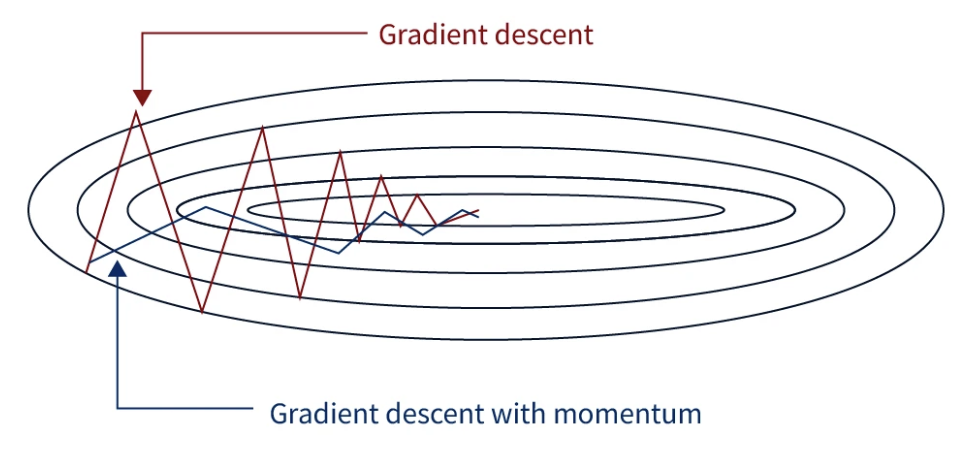
\includegraphics[scale=0.4]{figures/math/stochasticgradientdescent}
\caption{Stochastic Gradient Descent (SGD) Algorithm with and without Momentum}
\end{figure}

\begin{remark} \hlt{Nesterov Momentum}\\
Inspired by Nesterov's accelerated gradient method, the update rules are:
\begin{align}
\bm{v} &\leftarrow \alpha \bm{v} - \epsilon \nabla_{\bm{\theta}} \left(\frac{1}{m} \sum\limits_{i=1}^m L(\bm{f}(\bm{x}^{(i)}; \bm{\theta} + \alpha \bm{v}), \bm{y}^{(i)}) \right) \nonumber \\
\bm{\theta} &\leftarrow \bm{\theta} + \bm{v} \nonumber
\end{align}
Note, gradient is evaluated after current velocity is applied.\\
Hence, Nesterov momentum is adding a correction factor to the standard method of momentum.
\end{remark}

\begin{breakablealgorithm}
\caption{Stochastic Gradient Descent (SGD) with Nesterov Momentum}
\begin{algorithmic}
\Require \\
Learning rate $\epsilon_k$, Momentum parameter $\alpha$\\
Initial parameter $\bm{\theta}$, Initial velocity $\bm{v}$\\

\While {stopping criterion not met}
\State Sample a minibatch of $m$ samples from the training set $\{\bm{x}^{(1)}, \ldots, \bm{x}^{(m)} \}$ with targets $\bm{y}^{(i)}$
\State Apply interim update: $\tilde{\bm{\theta}} \leftarrow \bm{\theta} + \alpha \bm{v}$
\State Compute gradient (at interim point): $\bm{g} \leftarrow \frac{1}{m} \nabla_{\tilde{\bm{\theta}}} \sum_{i} L(f(\bm{x}^{(i)}; \tilde{\bm{\theta}}), \bm{y}^{(i)})$
\State Compute velocity update: $\bm{v} \leftarrow \alpha \bm{v} - \epsilon \bm{g}$
\State Apply update: $\bm{\theta} \leftarrow \bm{\theta} + \bm{v}$
\EndWhile
\end{algorithmic}
\end{breakablealgorithm}

\begin{figure}[H]
\centering
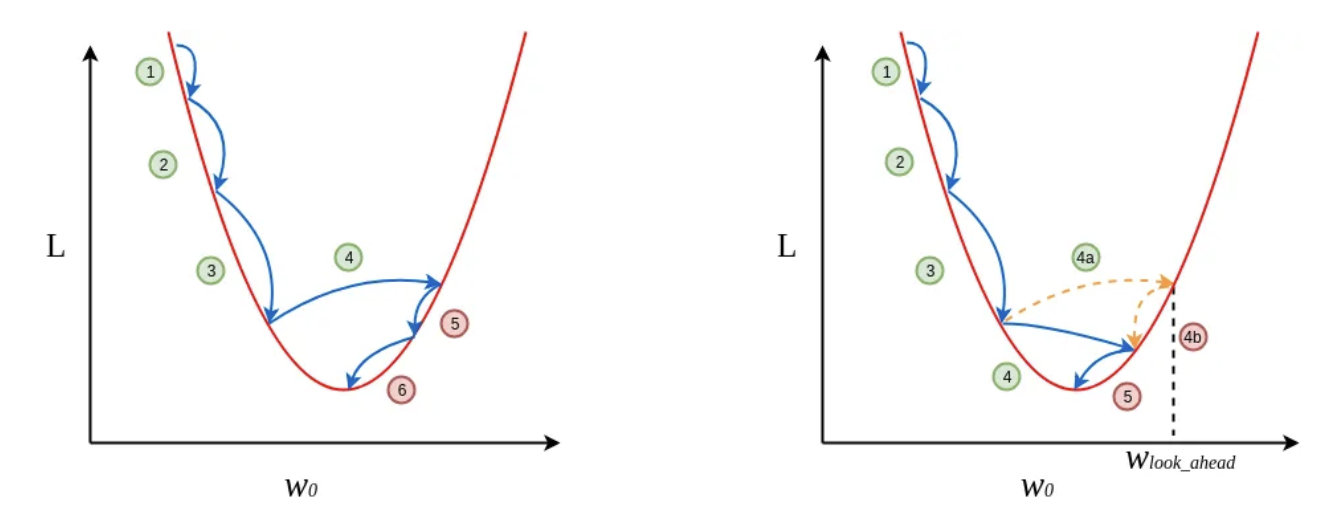
\includegraphics[scale=0.4]{figures/math/nesterov}
\caption{Momentum vs Nesterov Gradient Descent}
\end{figure}

\begin{remark} \hlt{Parameter Initialisation Challenges}\\
Training deep neural networks is difficult as most algorithms are strongly affected by choice of initialisation.\\
Designing initialisation strategies is difficult as neural network optimisation is not yet well understood, as the nice properties from initialisation may not be preserved as training proceeds.\\
Some initial points may be beneficial for optimisation, but detrimental for generalisation.
\end{remark}

\begin{remark} \hlt{Parameter Initialisation Strategies}\\
Initial parameters need to 'break symmetry' between different units. May explicitly search for large set of basis functions mutually different from each other, but this may incur noticeable computational cost.\\
Random initialisation from high-entropy distribution over high-dimensional space is computationally cheaper.\\
Larger initial weights will yield stronger symmetry breaking effect and avoid redundant units. However, if weights are set too large, may result in chaos (extreme sensitivity to small perturbations of input). Exploding gradient may be mitigated by gradient clipping. The bias (i.e., parameters encoding conditional variance of a prediction) for each unit is set to heuristically chosen constraints.
\end{remark}

\begin{remark} \hlt{Weight Initialisation Heuristics}\\
Initialising parameters of neural network $\bm{\theta}$ to $\bm{\theta}_0$ is similar to imposing a Gaussian prior $p(\bm{\theta})$ with mean $\bm{\theta}_0$, hence it make sense to choose $\bm{\theta}_0$ near $0$. Initialisation of $\bm{\theta}_0$ to large values means prior specifies which units should interact with each other, and how they should interact.\\
For a fully connected neural network with $m$ inputs and $n$ outputs, weights may be initialised by:
\begin{enumerate}[label=\roman*.]
\setlength{\itemsep}{0pt}
\item Sampling from $U\left(-\frac{1}{\sqrt{m}},  \frac{1}{\sqrt{m}} \right)$
\item Sampling from normalised initialisation $W_{i,j} \sim U \left(-\sqrt{\frac{6}{m+n}},  \sqrt{\frac{6}{m+n}} \right)$ (Glorot and Bengio). Compromise between goal of initialising all layers to have same activation variance and that of same gradient variance. Derived from assumption that network is chain of matrix multiplications with no nonlinearities.
\item Sampling from random orthogonal matrices, with scaling or gain factor $g$ that accounts for nonlinearity at each layer, with specific values for different types of nonlinear activation functions. Assumes neural network is sequence of matrix multiplications without nonlinearities. Guarantees the total number of training iterations required to reach convergence is independent of depth.\\
Increasing scaling factor $g$ pushes network toward regime where activations increase in norm in forward propagation, and gradients increase in norm in backward propagation.\\
For scaling rules that set all of initial weights to have same standard deviation, individual weight becomes extremely small when layers become large.
\item Sparse initialisation (Martens), where each unit is initialised to have exactly $k$ non-zero weight. Keep total number of input to unit independent from number of inputs $m$ without making magnitude of individual weight elements shrink with $m$.\\
Imposes very strong prior on weights that are chosen to have large Gaussian values.
\end{enumerate}
If computational resources allow, treat initial scale of weights for each layer as a hyper-parameter, and use hyper-parameter search algorithm. Choice of dense or sparse initialisation may also be a hyper-parameter.
\end{remark}

\begin{remark} \hlt{Bias Initialisation Heuristics}\\
Setting bias to zero is compatible with most weight initialisation schemes. The few other situations are:
\begin{enumerate}[label=\roman*.]
\setlength{\itemsep}{0pt}
\item If bias is for output unit, initialise bias to obtain right marginal statistics of the output. Assume initial weights are small enough that output of unit is determined only by bias. The bias will be inverse of activation function applied to marginal statistics of the output in training set.\\
If output is a highly skewed distribution over classes with marginal probability of class $i$ given by element $c_i$ of some vector $\bm{c}$, then bias vector $\bm{b}$ is such that $\text{softmax}(\bm{b}) = \bm{c}$. The models have output layers that should resemble input data $\bm{x}$, hence bias should match marginal distribution over $\bm{x}$.
\item If bias is to be set to avoid causing too much saturation at initialisation (i.e., with ReLU). Not compatible with weight initialisation schemes that do not expect strong input form bias (i.e., with random walk init).
\item If a unit controls whether other units are able to participate in a function. There is unit with output $u$ and another unit $h \in [0,1]$, multiplied together to produce output $uh$. Then $h$ is a gate that determines if $uh \approx u$ or $uh \approx 0$. Hence, to set bias for $h$ such that $h \approx 1$ at initialisation, else $u$ does not learn.
\end{enumerate}
\end{remark}

\begin{remark} \hlt{Variance or Precision Parameter Initialisation Heuristics}\\
For linear regression with conditional variance estimate using model
\begin{align}
p(y \ | \ \bm{x}) = \mathcal{N}(y \ | \ \bm{w}^T \bm{x} + b, 1/\beta) \nonumber
\end{align}
where $\beta$ is a precision parameter. The variance of precision parameters may be initialised to $1$.\\
Another approach is to assume initial weights are close enough to zero, and bias may be set while ignoring effect of the weights, then set bias to produce the correct marginal mean of the output, and set variance parameters to the marginal variance of the output in the training set.
\end{remark}

\begin{remark} \hlt{Model Parameter Initialisation with Machine Learning}\\
Initialise supervised model with parameters learned by unsupervised model trained on same inputs.\\
Alternatively, perform supervised training on a related task, which may yield initialisation that offers faster convergence than random initialisation. Information on distribution is encoded into initial parameters of model.
\end{remark}

\begin{remark} \hlt{Adaptive Gradient (AdaGrad) Algorithm}\\
Algorithm individually adapts learning rates of all model parameters by scaling them inversely proportional to square root of sum of all of their historical squared values. Has greater progress in more gently sloped directions of parameter space. On deep neural networks, accumulation of squared gradients from beginning of training can result in premature and excessive decrease in effective learning rate.
\end{remark}

\begin{breakablealgorithm}
\caption{Adaptive Gradient (AdaGrad) Algorithm}
\begin{algorithmic}
\Require \\
Global Learning rate $\epsilon$\\
Initial parameter $\bm{\theta}$\\
Small constant $\delta$, perhaps $10^{-7}$ for numerical stability\\

\State Initialise gradient accumulation variable $\bm{r} = \bm{0}$
\While {stopping criterion not met}
\State Sample a minibatch of $m$ samples from the training set $\{\bm{x}^{(1)}, \ldots, \bm{x}^{(m)} \}$ with targets $\bm{y}^{(i)}$
\State Compute gradient: $\bm{g} \leftarrow \frac{1}{m} \nabla_{\bm{\theta}} \sum_i L(f(\bm{x}^{(i)}; \bm{\theta}), \bm{y}^{(i)})$
\State Accumulate squared gradient: $\bm{r} \leftarrow \bm{r} + \bm{g} \odot \bm{g}$
\State Compute update: $\Delta \bm{\theta} \leftarrow - \frac{\epsilon}{\delta + \sqrt{\bm{r}}} \odot \bm{g}$ (Division and square root applied element-wise)
\State Apply update: $\bm{\theta} \leftarrow \bm{\theta} + \Delta \bm{\theta}$
\EndWhile
\end{algorithmic}
\end{breakablealgorithm}

\begin{remark} \hlt{Root Mean Squared Propagation (RMSProp) Algorithm}\\
Modifies AdaGrad to perform better in non-convex setting by changing gradient accumulation into exponentially weighted moving average, which discards history from extreme past so it can converge rapidly after finding a convex bowl. Use of moving average introduces a new hyper-parameter $\rho$ that controls length scale of the moving average. RMSProp is effective and practical for deep neural networks.
\end{remark}

\begin{breakablealgorithm}
\caption{Root Mean Squared Propagation (RMSProp) Algorithm}
\begin{algorithmic}
\Require \\
Global Learning rate $\epsilon$\\
Decay rate $\rho$\\
Initial parameter $\bm{\theta}$\\
Small constant $\delta$, perhaps $10^{-6}$ to stabilise division by small numbers\\

\State Initialise accumulation variable $\bm{r} = \bm{0}$
\While {stopping criterion not met}
\State Sample a minibatch of $m$ samples from the training set $\{\bm{x}^{(1)}, \ldots, \bm{x}^{(m)} \}$ with targets $\bm{y}^{(i)}$
\State Compute gradient: $\bm{g} \leftarrow \frac{1}{m} \nabla_{\bm{\theta}} \sum_i L(f(\bm{x}^{(i)}; \bm{\theta}), \bm{y}^{(i)})$
\State Accumulate squared gradient: $\bm{r} \leftarrow \rho \bm{r} + (1 - \rho) \bm{g} \odot \bm{g}$
\State Compute update: $\Delta \bm{\theta} \leftarrow - \frac{\epsilon}{\sqrt{\delta + \bm{r}}} \odot \bm{g}$ ($\frac{\epsilon}{\sqrt{\delta + \bm{r}}}$ applied element-wise)
\State Apply update: $\bm{\theta} \leftarrow \bm{\theta} + \Delta \bm{\theta}$
\EndWhile
\end{algorithmic}
\end{breakablealgorithm}

\begin{breakablealgorithm}
\caption{Root Mean Squared Propagation (RMSProp) Algorithm}
\begin{algorithmic}
\Require \\
Global Learning rate $\epsilon$\\
Decay rate $\rho$\\
Momentum coefficient $\alpha$\\
Initial parameter $\bm{\theta}$\\
Initial velocity $\bm{v}$\\

\State Initialise accumulation variable $\bm{r} = \bm{0}$
\While {stopping criterion not met}
\State Sample a minibatch of $m$ samples from the training set $\{\bm{x}^{(1)}, \ldots, \bm{x}^{(m)} \}$ with targets $\bm{y}^{(i)}$
\State Compute interim update $\tilde{\bm{\theta}} \leftarrow \bm{\theta} + \alpha \bm{v}$
\State Compute gradient: $\bm{g} \leftarrow \frac{1}{m} \nabla_{\tilde{\bm{\theta}}} \sum_i L(f(\bm{x}^{(i)}; \tilde{\bm{\theta}}), \bm{y}^{(i)})$
\State Accumulate gradient: $\bm{r} \leftarrow \rho \bm{r} + (1 - \rho) \bm{g} \odot \bm{g}$
\State Compute velocity update: $\bm{v} \leftarrow \alpha \bm{v} - \frac{\epsilon}{\sqrt{\bm{r}}} \odot \bm{g}$ ($\frac{1}{\sqrt{\bm{r}}}$ applied element-wise)
\State Apply update: $\bm{\theta} \leftarrow \bm{\theta} + \bm{v}$
\EndWhile
\end{algorithmic}
\end{breakablealgorithm}

\begin{remark} \hlt{Adaptive Moment Estimation (Adam) Algorithm}\\
Variant on combination of RMSProp and momentum. Note, momentum is incorporated directly as an estimate of first order moment of gradient; bias corrections are made to estimates of both first-order moments and second-order moments to account for initialisation at origin.\\
Algorithm is fairly robust to choice of hyper-parameters.
\end{remark}

\begin{breakablealgorithm}
\caption{Adaptive Moment Estimation (Adam) Algorithm}
\begin{algorithmic}
\Require \\
Step size $\epsilon$ (Suggested default: $0.001$)\\
Exponential decay rates for moment estimates $\rho_1, \rho_2$ in $[0,1)$ (Suggested defaults: $0.9$ and $0.999$)\\
Small constant $\delta$ used for numerical stabilisation (Suggested default: $10^{-8}$)\\
Initial parameters $\bm{\theta}$\\

\State Initialise $1$st and $2$nd momentum variables $\bm{s} = \bm{0}$, $\bm{r} = \bm{0}$
\State Initialise time step $t=0$
\While {stopping criterion not met}
\State Sample a minibatch of $m$ samples from the training set $\{\bm{x}^{(1)}, \ldots, \bm{x}^{(m)} \}$ with targets $\bm{y}^{(i)}$
\State Compute gradient: $\bm{g} \leftarrow \frac{1}{m} \nabla_{\bm{\theta}} \sum_i L(f(\bm{x}^{(i)}; \bm{\theta}), \bm{y}^{(i)})$
\State Update time step $t \leftarrow t+1$
\State Update biased first and second moment estimate: $\bm{s} \leftarrow \rho_1 \bm{s} + (1-\rho_1) \bm{g}$ and $\bm{r} \leftarrow \rho_2 \bm{r} + (1-\rho_2) \bm{g} \odot \bm{g}$
\State Correct bias in first and second moment: $\hat{\bm{s}} \leftarrow \frac{\bm{s}}{1 - \rho_1^t}$ and $\hat{\bm{r}} \leftarrow \frac{\bm{r}}{1 - \rho_2^t}$
\State Compute update: $\Delta \bm{\theta} = - \epsilon \frac{\hat{\bm{s}}}{\sqrt{\hat{\bm{r}} + \delta}}$ (Operations applied element-wise)
\State Apply update: $\bm{\theta} \leftarrow \bm{\theta} + \Delta \bm{\theta}$
\EndWhile
\end{algorithmic}
\end{breakablealgorithm}

\begin{remark} \hlt{Newton's Method}\\
Based on second-order Taylor's series approximating $J(\bm{\theta})$ near the point $\bm{\theta}_0$, ignoring higher derivatives
\begin{equation}
J(\bm{\theta}) \approx J(\bm{\theta}_0) + (\bm{\theta} - \bm{\theta}_0)^T \nabla_{\bm{\theta}} J(\bm{\theta}_0) + \frac{1}{2} (\bm{\theta} - \bm{\theta}_0)^T \bm{H}(\bm{\theta} - \bm{\theta}_0) \nonumber
\end{equation}
where $\bm{H}$ is the Hessian of $J$ with respect to $\bm{\theta}$ evaluated at $\bm{\theta}_0$.\\
Solving for critical point will get the Newton parameter update rule
\begin{equation}
\bm{\theta}^{*} = \bm{\theta}_0 - \bm{H}^{-1} \nabla_{\bm{\theta}} J(\bm{\theta}_0) \nonumber
\end{equation}
Note that for deep learning, the surface of objective function is non-convex. Regularising the Hessian will solve many of the issues such as saddle points etc.
\begin{equation}
\bm{\theta}^{*} = \bm{\theta}_0 - [H(f(\bm{\theta}_0)) + \alpha \bm{I}]^{-1} \nabla_{\bm{\theta}} J(\bm{\theta}_0) \nonumber
\end{equation}
Due to requirement for inversion of the $k \times k$ matrix with time complexity $O(k^3)$ at every training iteration, only networks with very small number of parameters may be trained with this method.
\end{remark}

\begin{breakablealgorithm}
\caption{Newton's Method with Objective $J(\bm{\theta}) = \frac{1}{m} \sum_{i=1}^m L(f(\bm{x}^{(i)}; \bm{\theta}), y^{(i)})$}
\begin{algorithmic}
\Require \\
Initial parameter $\bm{\theta}_0$\\
Training set of $m$ examples\\

\While {stopping criterion not met}
\State Compute gradient $\bm{g} \leftarrow \frac{1}{m} \nabla_{\bm{\theta}} \sum_i L(f(\bm{x}^{(i)}; \bm{\theta}), \bm{y}^{(i)})$
\State Compute Hessian: $\bm{H} \leftarrow \frac{1}{m} \nabla_{\bm{\theta}}^2 \sum_i L(f(\bm{x}^{(i)}; \bm{\theta}), \bm{y}^{(i)})$
\State Compute Hessian Inverse: $\bm{H}^{-1}$
\State Compute update: $\Delta \bm{\theta} = - \bm{H}^{-1} \bm{g}$
\State Apply update: $\bm{\theta} \leftarrow \bm{\theta} + \Delta \bm{\theta}$
\EndWhile
\end{algorithmic}
\end{breakablealgorithm}

\begin{remark} \hlt{Conjugate Gradient Method}\\
Method effectively avoids computation of inversion Hessian by descending conjugate directions, which is a search direction conjugate to the previous line search direction (will not undo progress made in that direction).\\
Let current and previous search directions be $\bm{d}_{t}, \bm{d}_{t-1}$. At training iteration $t$, the next search direction $\bm{d}_t$ is
\begin{equation}
\bm{d}_t = \nabla_{\bm{\theta}} J(\bm{\theta}) + \beta_t \bm{d}_{t-1} \nonumber
\end{equation}
note that $\beta_t$ may be computed via Fletcher Reeves:
\begin{equation}
\beta_t = \frac{\nabla_{\bm{\theta}} J(\bm{\theta}_t)^T \nabla_{\bm{\theta}} J(\bm{\theta}_t)}{\nabla_{\bm{\theta}} J(\bm{\theta}_{t-1})^T \nabla_{\bm{\theta}} J(\bm{\theta}_{t-1})} \nonumber
\end{equation}
or may be computed with Polak-Ribiere:
\begin{equation}
\beta_t = \frac{(\nabla_{\bm{\theta}} J(\bm{\theta}_t) - \nabla_{\bm{\theta}} J(\bm{\theta}_{t-1}))^T \nabla_{\bm{\theta}} J(\bm{\theta}_t)}{\nabla_{\bm{\theta}} J(\bm{\theta}_{t-1})^T \nabla_{\bm{\theta}} J(\bm{\theta}_{t-1})} \nonumber
\end{equation}
The non-linear conjugate gradient method is a variation which uses occasional resets where the method is restarted with line search along with the unaltered gradient.
\end{remark}

\begin{breakablealgorithm}
\caption{Conjugate Gradient Method}
\begin{algorithmic}
\Require \\
Initial parameter $\bm{\theta}_0$\\
Training set of $m$ examples\\
Initialise $\bm{\rho}_0 = 0$\\
Initialise $g_0 = 0$\\
Initialise $t = 1$\\

\While {stopping criterion not met}
\State Initialise the gradient $\bm{g}_t = \bm{0}$
\State Compute gradient $\bm{g} \leftarrow \frac{1}{m} \nabla_{\bm{\theta}} \sum_i L(f(\bm{x}^{(i)}; \bm{\theta}), \bm{y}^{(i)})$
\State Compute Polak-Ribiere metric: $\beta_t = \frac{(\bm{g}_t - \bm{g}_{t-1})^T \bm{g}_t}{\bm{g}_{t-1}^T \bm{g}_{t-1}}$
\State (Nonlinear conjugate gradient: optionally reset $\beta_t = 0$, i.e., if $t$ is a multiple of some constant $k$)
\State Compute search direction: $\bm{\rho}_t = -\bm{g}_t + \beta_t \bm{\rho}_{t-1}$
\State Perform line search to find: $\epsilon^{*} = \arg \min_{\epsilon} \frac{1}{m} \sum_{i=1}^m L(f(\bm{x}^{(i)}; \bm{\theta}_t + \epsilon \bm{\rho}_t), \bm{y}^{(i)})$
\State (On truly quadratic cost function, analytically solve for $\epsilon^{*}$)
\State Apply update: $\bm{\theta}_{t+1} = \bm{\theta}_{t} + \epsilon^{\theta} \bm{\rho}_t$
\State Apply time step $t \leftarrow t + 1$
\EndWhile
\end{algorithmic}
\end{breakablealgorithm}

\begin{remark} \hlt{Nonlinear Conjugate Gradients}\\
Method of conjugate gradients is still applicable for non-linear objective function.\\
Conjugate directions are no longer assumed to remain at minimum of the objective for previous directions. Has occasional resets where method of conjugate gradients is restarted with line search along unaltered gradient.
\end{remark}

\begin{remark} \hlt{Broyden-Fletcher-Goldfarb-Shanno (BGFS) Algorithm}\\
Similar to conjugate gradient, but uses more direct approach to approximation of newton's update.\\
Method approximate the inverse of hessian $\bm{H}$ with matrix $\bm{M}_t$, iteratively refined by low rank updates to better approximate $\bm{H}^{-1}$. Direction of gradient descent is then determined by $\bm{\rho}_t = \bm{M}_t \bm{g}_t$. Line search is performed in this direction to determine step size $\epsilon^{*}$. Final update of parameter is then $\bm{\theta}_{t+1} = \bm{\theta}_t + \epsilon^{*} \bm{\rho}_{t}$.\\
Note, BGFS store matrix $\bm{M}$ which requires $O(n^2)$ memory, making it impractical for most modern models.
\end{remark}

\begin{remark} \hlt{Limited Memory BFGS (L-BFGS) Algorithm}\\
Memory costs of BFGS may be decreased by not storing complete inverse Hessian approximation $\bm{M}$. L-BFGS computes approximation $\bm{M}$ with same method as BFGS, but assumes at beginning that $\bm{M}^{(t-1)}$ is the identity matrix, rather than storing the approximation between steps.\\
If used with exact line searches, directions defined by L-BFGS are mutually conjugate, and this procedure remains well-behaved when minimum of line search is reached only approximately.\\
L-BFGS may be generalised to store some vectors used to update $\bm{M}$ at each time step, costing $O(n)$ per step.
\end{remark}

\begin{remark} \hlt{Meta-Algorithm: Batch Normalisation}\\
An update from optimisation algorithm may result in multiple-order effects, and in very deep networks, even higher-order interactions can be significant.\\
Batch normalisation provides an elegant way of re-parametrising any deep network, which reduces the problem of coordinating updates across multiple layers. Batch normalisation may be applied to any input/hidden layer.\\
Let $\bm{H}$ be minibatch of activations of layer to normalise, with activations for each example appearing in a row. To normalise $\bm{H}$, replace it with $\bm{H}' = \frac{\bm{H} - \bm{\mu}}{\bm{\sigma}}$ where $\bm{\mu}$ is a vector of mean of each unit and $\sigma$ is a vector of standard deviation of each unit. Then $H_{ij}$ is normalised by subtracting $\mu_j$ and dividing $\sigma_j$. Rest of network then operates on $\bm{H}'$ just as in original network on $\bm{H}$.\\
At training, the mean and standard deviations are computed as
\begin{align}
\bm{\mu} &= \frac{1}{m} \sum\limits_i \bm{H}_{i, ;}, \ \ \ \bm{\sigma} = \sqrt{\delta + \frac{1}{m} \sum\limits_{i} (\bm{H} - \bm{\mu})^2_i} \nonumber
\end{align}
where $\delta$ is a small positive value (i.e., $10^{-8}$) to avoid undefined gradient of $\sqrt{z}$ at $z=0$.\\
These are then back-propagated to normalise $\bm{H}$, hence gradient will never increase the standard deviation or mean of $h_i$. Batch normalisation re-parametrises the model to make some units always standardised.\\
At test time, $\mu$ and $\sigma$ may be replaced by running averages from training time. This allows model to be evaluated on a single example, without needing to use definitions of $\mu$ and $\bm{\sigma}$ that depends on entire minibatch.
\end{remark}

\begin{remark} \hlt{Batch Normalisation but Maintain Network Express Power}\\
Replace batch of hidden activations $\bm{H}$ with $\bm{\gamma} \bm{H}' + \bm{\beta}$ rather than $\bm{H}'$, where $\bm{\gamma}$ and $\bm{\beta}$ are learned parameters to allow new variable to have any mean and standard deviation. With original $\bm{H}'$, mean of $\bm{H}$ was determined by complicated interaction between parameters in layers below $\bm{H}$. With $\bm{\gamma} \bm{H}' + \bm{\beta}$, the mean is determined solely by $\bm{\beta}$, which is much easier to learn with gradient descent.\\
Most neural network layers are of form $\phi(\bm{X} \bm{W} + \bm{b})$, where $\phi$ is some fixed nonlinear activation function. Then $\bm{X} \bm{W} + \bm{b})$ should be replaced by normalised version of $\bm{X} \bm{W}$, and bias term omitted as it becomes redundant with $\beta$ parameter applied from batch normalisation re-parametrisation. Statistics of input are non-Gaussian and less amenable to standardisation by linear operations.	
\end{remark}

\begin{remark} \hlt{Meta-Algorithm: Coordinate Descent}\\
Solving optimisation problems by minimising the objective function $f(\bm{x})$ with respect to a single variable $x_i$, and rapidly cycling through all variables. \hlt{Block coordinate descent} refers to minimising with respect to a subset of variables simultaneously.\\
 Coordinate descent works when different variables can be clearly separated into groups that play relatively isolated roles, or when optimisation with respect to one group of variables is significantly more efficient than optimisation with respect to all of the variables.
\end{remark}

\begin{example} \hlt{Sparse Encoding with Coordinate Descent}\\
Consider the cost function
\begin{align}
J(\bm{H}, \bm{W}) = \sum\limits_{i,j} \abs{H_{ij}} + \sum\limits_{i,j} (\bm{X} - \bm{W}^T \bm{H})^2_{i,j} \nonumber
\end{align}
To find weight matrix $\bm{W}$ that can linearly decode a matrix of activation values $\bm{H}$ to reconstruct training set $\bm{X}$. Most applications also include weight decay or constraint on norms of columns of $\bm{W}$ to prevent the pathological solution with extremely small $\bm{H}$ and large $\bm{W}$.\\
Note $J$ is not convex, but inputs may be divided into the dictionary parameters $\bm{W}$ and the code representations $\bm{H}$. Minimising object function with respect to either set is a convex problem.
\end{example}

\begin{remark} \hlt{Polyak Averaging}\\
Average several points in trajectory through parameter space visited by optimisation algorithm.\\
If $t$ iterations of gradient descent visit points $\bm{\theta}^{(1)}, \ldots, \bm{\theta}^{(t)}$, then the output is $\hat{\bm{\theta}}^{(t)} = \frac{1}{t} \sum_i \bm{\theta}^{(i)}$.\\
The optimisation algorithm may leap back and forth across a valley several times without visiting the minimum point, and the average of all points on either side of the valley should be close to minimum value.\\
This is developed solely for stochastic gradient descent (SGD) to stabilise the estimates (\cite{granziol2020gadam}).\\
For non-convex problems, an exponentially decaying running average is used:
\begin{align}
\hat{\bm{\theta}}^{(t)} = \alpha \hat{\bm{\theta}}^{(t-1)} + (1- \alpha)\bm{\theta}^{(t)} \nonumber
\end{align}
\end{remark}

\begin{remark} \hlt{Supervised Pre-training}\\
Pre-training refers to training simple models on simple tasks before training the desired model on desired task.\\
Greedy algorithms break problem into many components, then solve for optimal version of each component in isolation, which is must cheaper than algorithms that solve for best joint solution. Fine-tuning on joint optimisation algorithm searches for optimal solution to the full problem.\\
Greedy supervised training breaks supervised learning problems into other simpler supervised learning problems.\\
Transfer learning refers to pre-training a deep network on a set of tasks, then initialise a same-size network with first $k$ layers of first net. The layers of second networks (upper layers initialised randomly) are then jointly trained to perform a different set of tasks with fewer training examples than for first set of tasks.\\
FitNets approach begins by training a network with low depth and high width, which becomes a teacher for a second network (the student), which is much deeper and thinner. Student network is trained to not only predict the output on original task, but also on value of middle layer of teacher network.
\end{remark}

\begin{remark} \hlt{Neural Network Design Choice: Linear Transformation}\\
Model units have generally moved towards using more linear functions, which allow model to have nice properties that make optimisation easier. The model's local gradient information corresponds reasonably well to moving towards a distant solution.
\end{remark}

\begin{remark} \hlt{Neural Network Design Choice: Linear Paths and Skip Connections}\\
Linear paths and skip connections between layers reduce length of shortest path from lower layer's parameters to the output, mitigating vanishing gradient problem.\\
Adding extra copies of output that are attached to intermediate hidden layers is an alternative to pre-training, where these 'auxiliary heads' are trained to perform the same task as primary output at the top of the network to ensure that the lower layers receive a large gradient. After training, these may be discarded.
\end{remark}

\begin{remark} \hlt{Continuation Methods}\\
Family of strategies that can make optimisation easier by choosing initial points to ensure that local optimisation spends most of its time in well-behaved regions. Method constructs series of objective functions $\{J^{(0)}, \ldots, J^{(n)}\}$ which are increasingly difficult to minimise (well-behaved over less regions of $\bm{\theta}$ space) for the true cost function $J(\bm{\theta})$. The cost functions are designed such that a solution to one is a good initial point for the next.\\
Continuation methods aim to reach a global minimum despite many local minima. Easier cost functions are constructed through the blurring operation, which approximates
\begin{align}
J^{(i)}(\bm{\theta}) = \mathbb{E}_{\theta' \sim \mathcal{N}(\bm{\theta}'; \bm{\theta}, \sigma^{(i)2})} J(\bm{\theta})' \nonumber
\end{align}
via sampling. Some non-convex functions become approximately convex when blurred, but preserved enough information about local global minimum. However, approach might not work when
\begin{enumerate}[label=\roman*.]
\setlength{\itemsep}{0pt}
\item so many incremental cost functions are required that cost of entire procedure remains high;
\item NP-hard optimisation problems remain NP-hard, even when continuation methods are applicable;
\item function might not become convex, no matter how much it is blurred;
\item function may become convex due to blurring, but minimum of this blurred function may track a local rather than global minimum of original cost function.
\end{enumerate}
\end{remark}

\begin{remark} \hlt{Curriculum Learning}\\
Planning a learning process to begin by learning simple concepts, and progress to learning more complex topics that depend on these simpler concepts. Earlier objective functions $J^{(i)}$ are made easier by increasing the influence of simpler examples.\\
Stochastic curriculum is a variation of the approach where a random mix of easy and difficult examples is always presented to the learner, but average proportion of more difficult examples is gradually increased.
\end{remark}
